\section[对权重的依赖]{对权重的依赖\\Dependency on the Weights}
\begin{flushleft}
	$A$ person who has gained a basic knowledge of least-squares problems soon asks the question: How important are the weights? If we change them a little how much does this change the solution? Let us try to get some insight to the problem. As usual we start by a set of observation equations $ A\textbf{\textit{x}}=\textbf{\textit{b}}-\textbf{\textit{e}} $ and with weight matrix $C$.
\end{flushleft}

We separate the observation vector $\textbf{\textit{b}}$ into two subvectors. At first we put no restrictions on the dimensions of $\textbf{\textit{b}}_{1}$ and $\textbf{\textit{b}}_{2}$. The vector $\textbf{\textit{e}}$ and matrix $A$ and weight $C$ are
\begin{align*}
\textbf{\textit{b}}=
\begin{bmatrix}
\textbf{\textit{b}}_{1} \\	
\textbf{\textit{b}}_{2}
\end{bmatrix},
\quad
\textbf{\textit{e}}=
\begin{bmatrix}
\textbf{\textit{e}}_{1} \\	
\textbf{\textit{e}}_{2}
\end{bmatrix},
\quad
A=
\begin{bmatrix}
A_{1} \\	
A_{2}
\end{bmatrix},
\quad
C=
\begin{bmatrix}
C_{1} & 0\\	
  0   & C_{2}
\end{bmatrix}.
\end{align*}
\begin{flushleft}
	This means there is no weight coupling between the two groups of observations. The original problem becomes two distinct problems:
\end{flushleft}
\begin{align*}
A_{1}\textbf{\textit{x}}&=\textbf{\textit{b}}_{1}-\textbf{\textit{e}}_{1}  &\text{with \ weight \ matrix} \ C_{1}                      \\
A_{2}\textbf{\textit{x}}&=\textbf{\textit{b}}_{2}-\textbf{\textit{e}}_{2}  &\text{with \ weight \ matrix} \ C_{2}    
\end{align*}
\begin{flushleft}
	and we can calculate the solution of each system. Now the interesting question is: \textit{How do these solutions behave compared to the solution of the total problem}?
\end{flushleft}

We shall see how the solution $\hat{\textbf{\textit{x}}}$ is changed by $ \delta \textbf{\textit{x}} $ when we change the weights $C_{2}$ of the second group to $ C_{2}+\delta C_{2}$. The expression for $ \delta \textbf{\textit{x}}$ involves matrix calculations leading to a useful matrix formula.The normal equation for the original, total problem is

\begin{align*}
\begin{bmatrix}
A^{T}_{1} &	A^{T}_{2}
\end{bmatrix}
\begin{bmatrix}
C_{1} &	0 \\
0     &	C_{2}
\end{bmatrix}
\begin{bmatrix}
A_{1} \\
A_{2}
\end{bmatrix}  \hat{\textbf{\textit{x}}} = 
\begin{bmatrix}
A^{T}_{1} &	A^{T}_{2}
\end{bmatrix}
\begin{bmatrix}
C_{1} &	0 \\
0     &	C_{2}
\end{bmatrix}
\begin{bmatrix}
\textbf{\textit{b}}_{1} \\
\textbf{\textit{b}}_{2}
\end{bmatrix}.
\end{align*}
\begin{flushleft}
	This can he written as
\end{flushleft}
\begin{align}
(A^{T}_{1}C_{1}A_{1}+A^{T}_{2}C_{2}A_{2})\hat{\textbf{\textit{x}}}=A^{T}_{1}C_{1}\textbf{\textit{b}}_{1}+A^{T}_{2}C_{2}\textbf{\textit{b}}_{2}.
\end{align}
\begin{flushleft}
	Notice how the normal equations from the two problems have been collected. \textit{Contributions to the normal equation possess an additive character}. The perturbed problem is
\end{flushleft}
\begin{align}
(A^{T}_{1}C_{1}A_{1}+A^{T}_{2}(C_{2}+\delta C_{2} )A_{2})(\hat{\textbf{\textit{x}}}+\delta \textbf{\textit{x}} )=(A^{T}_{1}C_{1}\textbf{\textit{b}}_{1}+A^{T}_{2}(C_{2}+\delta C_{2} )\textbf{\textit{b}}_{2}).
\end{align}
\begin{flushleft}
	Now subtract (6.31) from (6.32) to find an equation for $ \delta \textbf{\textit{x}} $:
\end{flushleft}
\begin{align}
(A^{T}_{1}C_{1}A_{1}+A^{T}_{2}(C_{2}+\delta C_{2} )A_{2})\delta \textbf{\textit{x}} + A^{T}_{2}\delta C_{2}A_{2}\textbf{\textit{x}}=
A^{T}_{2}\delta C_{2}\textbf{\textit{b}}_{2}.
\end{align}
\begin{flushleft}
	We set  $ N= A^{T}_{1}C_{1}A_{1} + A^{T}_{2}C_{2}A_{2}$ and $ \hat{\textbf{\textit{e}}}_{2} = \textbf{\textit{b}}_{2} - A_{2}\textbf{\textit{x}}  $. Then the change in $\hat{\textbf{\textit{x}}}$ is
\end{flushleft}
\begin{align}
\delta \textbf{\textit{x}} = ( N + A^{T}_{2}\delta C_{2}A_{2})^{-1}
A^{T}_{2}\delta C_{2} \hat{\textbf{\textit{e}}}_{2}.
\end{align}
\begin{flushleft}
	The following important formula, taken from (8.45), yields the change in the inverse:
\end{flushleft}
\begin{align}
( N + A^{T}_{2}\delta C_{2}A_{2})^{-1} = N^{-1} - N^{-1}A^{T}_{2}
(A_{2}N^{-1}A^{T}_{2} +(\delta C_{2})^{-1} )^{-1} A_{2} N^{-1}
\end{align}
\begin{flushleft}
	For $n$ observations, this matrix multiplies  $ A^{T}_{2}\delta C_{2} \hat{\textbf{\textit{e}}}_{2} $ to give  $ \delta \textbf{\textit{x}} $. If we specialize to one single observation, $ A^{T}_{2} $ becomes an $n$ by 1 matrix and  $ \delta C_{2} $ is 1 by 1. We name the product  $ A_{2}N^{-1}A^{T}_{2} = s $ and get
\end{flushleft}
\begin{align*}
\delta \textbf{\textit{x}} = N^{-1} A^{T}_{2} (1-\dfrac{\delta C_{2}}{1+s\delta C_{2}}s)\delta C_{2}\hat{e}_{2}
\end{align*}
or
\begin{align}
\delta \textbf{\textit{x}} = \dfrac{\hat{e}_{2}\delta C_{2} }{1+s\delta C_{2}}N^{-1}A^{T}_{2}.
\end{align}
The expression (6.36) reveals several interesting facts. The change  $ \delta \textbf{\textit{x}} $  in the solution (in a first order approximation) is proportional to the change of weight $ \delta C_{2} $. The change $ \delta \textbf{\textit{x}} $ increases most in the unknowns which are connected to the observations contained in $A_{2}$. The product $ N^{-1}A^{T}_{2} $ only has contributions from the columns in $N^{-1}$ which corresponds to entries in $ A^{T}_{2} $ different from zero.

Already in 1823 C. F. Gauss found a similar expression for changes of a single weight $ \delta C_{2} $. See the section "Updating the unknowns of an observation changes" in Gauss (1995).
\begin{figure}[htb]
	\centering
	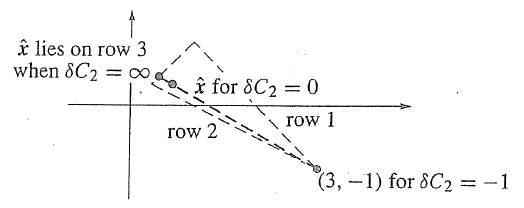
\includegraphics[width=0.7\linewidth]{TeX_files/Part02/chapter06/image/6-1}
	\caption{Dependence of $ \hat{\textbf{\textit{x}}}$ on $ \delta C_{2}$ in Example 6.4}
\end{figure}

\begin{flushleft}
	\textbf{Example 6.4} We want to demonstrate the procedure on a simple least-squares problem:
\end{flushleft}
\begin{align*}
	A = 
	\begin{bmatrix}
		1&1 \\	
		1&2 \\		
	   -1&1 	
	\end{bmatrix} \quad 
and \quad 
\textbf{\textit{b}}=
\begin{bmatrix}
	2 \\	
	1 \\		
	0 	
\end{bmatrix} \quad 
and \quad 
C+\delta C_{2} =
\begin{bmatrix}
	1   &   & \\	
	&   2   & \\		
	&   &  1+\delta C_{2} 	
\end{bmatrix} 
\end{align*}
Then $ \delta C_{2} =0 $ produces the solution $\hat{\textbf{\textit{x}}}$ and the residual vector $\hat{\textbf{\textit{e}}}$ as usual:
\begin{align*}
	\hat{\textbf{\textit{x}}} = \dfrac{1}{3}
\begin{bmatrix}
	2 \\	
	1 	
\end{bmatrix} \quad 
	and \quad 
\hat{\textbf{\textit{e}}} = \dfrac{1}{3}
	\begin{bmatrix}
		3 \\	
		-1 \\
		1	
	\end{bmatrix}.
\end{align*}
Setting $\delta C_{2} =-1 $ corresponds to eliminating the third observation. Then $ \hat{\textbf{\textit{x}}} =(3,-1)$ is the intersection point of the first two rows.  Varying $\delta C_{2} $ from -1 to $ \infty$ we get the line segment from (3,-1) to (5/11, 5/11) on the third row. \textit{Letting all weights vary, we evidently can obtain solutions anywhere in the interior of the triangle.}

The $M$-file $dw$ reflects what goes on.

This approach to changes of weight is excellent for a small number of obseiwations. For a more qualitative knowledge about a larger problem, we turn to a more powerful tool.

Now we ask for more quantitative results: If the weights are changed, how much can the projection $\textbf{\textit{p}}=P\textbf{\textit{b}}$ move in the column space of $A$? $A$ measure for this movement is
\begin{align}
tan \alpha = \dfrac{\rVert \textbf{\textit{p}}_{2} - \textbf{\textit{p}}_{1}\rVert c_{1}}{\rVert \textbf{\textit{b}} - \textbf{\textit{p}}_{1}\rVert c_{1}}.
\end{align}
The norm is weighted by $ \rVert \textbf{\textit{x}} \rVert c_{1}  = \rVert  C_{1}\textbf{\textit{x}} \rVert$ and $ \alpha$ is the angle at $\textbf{\textit{b}}$ which spans $ \overline{\textbf{\textit{p}}_{1}\textbf{\textit{p}}_{2}}$.Note that Figure 6.2 is drawn in $C_{1}$-norm. The angle at $\textbf{\textit{p}}_{2}$ is $C_{2}$ orthogonal; but in the $C_{1}$-norm the angle is $ \dfrac{\pi}{2} - \alpha$. The change from $C_{1}$ to $C_{2}$-norm leads to a change of the angle from $ \dfrac{\pi}{2}$ to $ \dfrac{\pi}{2} - \alpha$.

The square root $W$ of a matrix $C$ is the positive definite matrix that satisfies $W^{2}=C$. Such a matrix certainly exists, is unique, and nonsingular. We define $ D = W^{-1}_{1}C_{2}W^{-1}_{1}$, whose condition number $c(D)$-the ratio between the largest and smallest eigenvalue-can be related to the angle $ \alpha$:
\begin{align}
2\lvert tan\alpha \rvert \leq \sqrt{c(D)} - \dfrac{1}{\sqrt{c(D)}}.
\end{align}
\begin{figure}[!h]
	\centering
	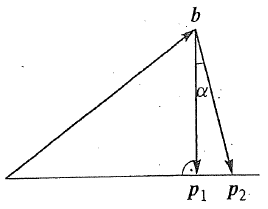
\includegraphics[height=0.23\linewidth]{TeX_files/Part02/chapter06/image/6-2}
	\caption{The dependence of the projection on the norm. The figure is drawn in $C_{1}$-norm.}
\end{figure}

\begin{flushleft}
	Let us repeat: $A$ least-squares problem is given by the coefficient matrix $A$, the weight $C_{0}$,and the observations $\textbf{\textit{b}}$. We consider all weight matrices $C$ such that the eigenvalues of $ W^{-1}_{0}CW^{-1}_{0}$ lie in the closed interval $[s,t]$. In the $C_{0}$-normwe always find
\end{flushleft}
\begin{align}
\lvert tan \alpha \rvert \leq \dfrac{1}{2} (\sqrt{\dfrac{t}{s}} - \sqrt{\dfrac{s}{t}}).
\end{align}
The angle $ \alpha$ measures the displacement of the least-squares result as seen from $\textbf{\textit{b}}$. At least one matrix $C$ exists for which the equality sign is valid. Furthermore, the ratio between the norms of the residual vectors corresponding to $C_{1}$ and $C_{2}$ is bounded by
\begin{align}
\dfrac{1}{\sqrt{\lambda_{max}}} \leq \dfrac{\rVert \textbf{\textit{b}} - \textbf{\textit{p}}_{1}\rVert c_{1}}{\rVert \textbf{\textit{b}} - \textbf{\textit{p}}_{2}\rVert c_{2}} \leq \sqrt{\lambda_{max}}
\end{align}
where $ \lambda_{max}$ is the largest eigenvalue of the matrix$ W^{-1}_{2}CW^{-1}_{2}$.

The main results about the changes of weight in a least-squares problem are quoted from Krarup (1972). Once again the condition number is prominent. We are saying that the effect of ignoring a possible correlation between the observations can be dangerous if the condition number is large.
\begin{flushleft}
	\textbf{Example 6.5} We introduce an $n$ by $ n$ covariance matrix with strong correlation:
\end{flushleft}
\begin{align*}
\Sigma_{b} =
\begin{bmatrix}
2    &    -1          &        &        & \\
-1   &     2    &    -1        &        & \\
&       \ddots  &  \ddots      & \ddots & \\
&          &         -1    &   2    &  -1 \\
&          &          &       -1    &   2
\end{bmatrix}.
\end{align*}
Its inverse has the special form
\begin{align*}
D = C_{2} = \Sigma^{-1}_{b} =
\left\{
\begin{aligned}
\dfrac{i(n+1-j)}{n+1} \quad \text{for} \ i\leq j\\
\dfrac{j(n+1-i)}{n+1} \quad \text{for} \ i\geq j.
\end{aligned}
\right.
\end{align*}
The eigenvalues are $ 4sin^{2} \dfrac{i\pi}{2(n+1)}$ so the condition is $ c(D) \approx \dfrac{4(n+1)^{2}}{\pi^{2}} < n^{2} $. By (6.39)
\begin{align*}
 \lvert tan \alpha \rvert \leq \dfrac{1}{2} ( \sqrt{c(D)} - \dfrac{1}{\sqrt{c(D)}}) \approx \dfrac{1}{\pi} (n+1) \rightarrow \infty.
\end{align*}
\begin{flushleft}
	A strong correlation can take us arbitrarily far from the solution corresponding to $C_{1}=I$.
\end{flushleft}
\begin{flushleft}
	\textbf{Example 6.6} The correlation is weaker if $ D = C_{2} = I +t\Sigma^{-1}_{b}$ and $ t \approx 10^{-2}$:
\end{flushleft}
\begin{align*}
c(D) = \dfrac{1+4sin^{2}\dfrac{n\pi}{2(n+1)}}{1+4sin^{2}\dfrac{\pi}{2(n+1)}} \approx 
(1+4t)(1-4t\dfrac{\pi^{2}}{4n^{2}}) \approx 1+4t.
\end{align*}
\begin{align*}
\lvert tan \alpha \rvert \leq \dfrac{1}{2} (\sqrt{1+4t} - \dfrac{1}{\sqrt{1+4t}}) = \dfrac{2t}{\sqrt{1+4t}}.
\end{align*}
Thus $\lvert tan \alpha \rvert < 2t $.